\documentclass[a4paper,11pt]{article}

\usepackage[dutch]{babel}
\usepackage{url}
\usepackage[latin1]{inputenc}
\usepackage{fullpage}
\usepackage{xspace}
\usepackage{graphicx}
\usepackage{float}
\usepackage{intcalc}

\usepackage{scrextend}
\usepackage{hyperref}
\usepackage[all]{hypcap}
\hypersetup{
    colorlinks=true,
    linkcolor=black,
    filecolor=magenta,      
    urlcolor=blue,
}
\urlstyle{same}

\renewcommand*{\figureautorefname}{figuur}
\renewcommand*{\sectionautorefname}{sectie}
\renewcommand*{\subsectionautorefname}{sectie}
\renewcommand*{\subsubsectionautorefname}{sectie} 

\newcommand{\one}{
\includegraphics[scale=0.5]{Gebruikershandleiding_img/1.png}}
\newcommand{\two}{
\includegraphics[scale=0.5]{Gebruikershandleiding_img/2.png}}
\newcommand{\three}{
\includegraphics[scale=0.5]{Gebruikershandleiding_img/3.png}}
\newcommand{\four}{
\includegraphics[scale=0.5]{Gebruikershandleiding_img/4.png}}
\newcommand{\five}{
\includegraphics[scale=0.5]{Gebruikershandleiding_img/5.png}}
\newcommand{\six}{
\includegraphics[scale=0.5]{Gebruikershandleiding_img/6.png}}
\newcommand{\seven}{
\includegraphics[scale=0.5]{Gebruikershandleiding_img/7.png}}
\newcommand{\eight}{
\includegraphics[scale=0.5]{Gebruikershandleiding_img/8.png}}
\newcommand{\nine}{
\includegraphics[scale=0.5]{Gebruikershandleiding_img/9.png}}
\newcommand{\ten}{
\includegraphics[scale=0.5]{Gebruikershandleiding_img/10.png}}
\newcommand{\eleven}{
\includegraphics[scale=0.5]{Gebruikershandleiding_img/11.png}}
\newcommand{\twelve}{
\includegraphics[scale=0.5]{Gebruikershandleiding_img/12.png}}
\newcommand{\thirteen}{
\includegraphics[scale=0.5]{Gebruikershandleiding_img/13.png}}
\newcommand{\fourteen}{
\includegraphics[scale=0.5]{Gebruikershandleiding_img/14.png}}

\newcommand*{\myitem}{
 \item[{\includegraphics[scale=0.5]{GebruikersHandleiding_img/\intcalcMod{\value{enumi}+1}{15}.png}}]\stepcounter{enumi}
}
\newcommand*{\myzeven}{
 \item[{\includegraphics[scale=0.5]{GebruikersHandleiding_img/\intcalcMod{\value{enumi}+7}{15}.png}}]\stepcounter{enumi}
}

\setlength{\parindent}{0em}
%\setlength{\parskip}{1em} zorgt voor vreemde lange inhoudstafel?

\begin{document}

\pagenumbering{roman}

\title{Gebruikershandleiding\\Vakoverschrijdend Project\\Groep 1}
\author{Mathias De Brouwer\\ Harm Delva\\ Maxime Fern\'andez Alonso\\ Jens Spitaels\\ Casper Van Gheluwe\\ Steven Van Maldeghem\\ Titouan Vervack}
\date{}
\maketitle
\tableofcontents
\pagenumbering{arabic}

\section{Inloggen}
\label{sec:login}
Bij het openen van de website (\url{http://vopro1.ugent.be/app}), komt u terecht op het inlogscherm.

\begin{figure}[H]
\centering
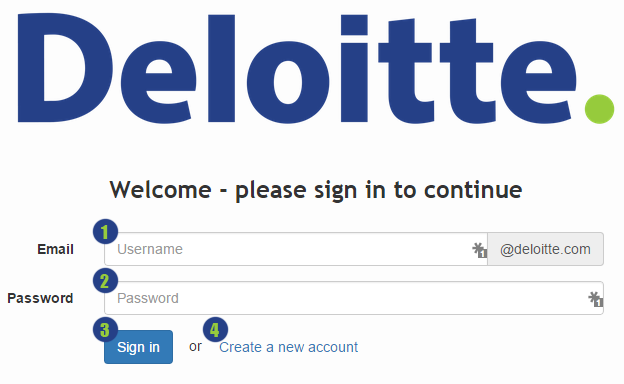
\includegraphics[scale=0.5]{Gebruikershandleiding_img/login.png}
\caption{Het inlogscherm van de webapplicatie}
\label{fig:login}
\end{figure}

\subsection{Reeds geregistreerd}
Indien u reeds geregistreerd bent als gebruiker, vult u bij \one\ uw gebruikersnaam en bij \two\ uw wachtwoord in en klikt u op $Sign\ in$ (\three), om in te loggen.\\
Ga naar \autoref{sec:teamlid} om verder te gaan.

\subsection{Een nieuwe account}
Indien u nog niet reeds geregistreerd bent, klikt u op $Create\ a\ new\ account$ (\autoref{fig:login}: \four) om een nieuwe account aan te maken.

\begin{figure}[H]
\centering
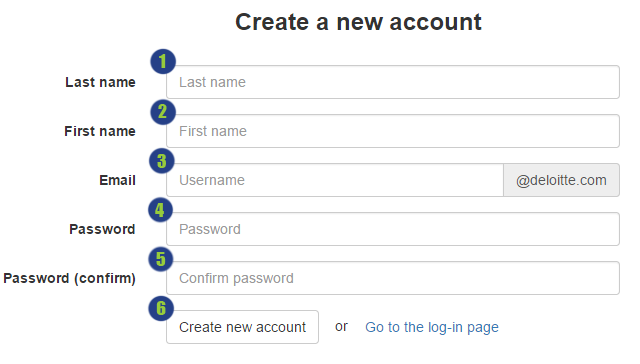
\includegraphics[scale=0.5]{Gebruikershandleiding_img/register.png}
\caption{Het registreren van een nieuwe gebruiker}
\label{fig:register}
\end{figure}

Nu ziet u het scherm op \autoref{fig:register}. Vul uw gegevens in op puntjes \one, \two\ en \three. Let op dat u enkel kan registreren met een Deloitte email adres. Geef vervolgens het wachtwoord in dat u wenst te gebruiken (\four) en herhaal dit wachtwoord bij puntje \five. Wanneer u op $Create\ new\ account$ (\six) klikt zal u zich als nieuwe gebruiker registreren.

\section{Algemeen}
Alle namen in de applicatie (gebruikers, projecten, teams, actoren, concepten, \ldots) zijn hoofdlettergevoelig, dit wil dus zeggen dat bijvoorbeeld '$Gebruiker1$' en '$gebruiker1$' 2 verschillende gebruikers zijn.\\
Ook zijn namen van entiteiten (usecases, actoren en concepten) uniek binnen een project. Dit wil zeggen dat er bijvoorbeeld in \'e\'en project geen actor 'Systeem' en een concept 'Systeem' kan bestaan.

\subsection{Permissies}
\label{subsec:permissions}
Zowel de applicatie als deze gebruikershandleiding steunen op het permissiesysteem. Er zijn gebruikers, teamleden, projectanalysten, usecase-analysten, projectleiders, teamleiders en administrators.\\
Iedereen kan een account aanmaken (gebruiker), maar deze krijgt pas nut indien de gebruiker wordt toegevoegd aan een team. E\'enmaal toegevoegd aan een team, wordt deze gebruiker een teamlid. Een teamlid kan van alle projecten van zijn team de inhoud lezen, maar hij kan niets aanpassen of nieuw aanmaken.\\
Een team wordt aangemaakt door een admin, bij het aanmaken van een team wordt een gebruiker aangesteld als teamleider. Deze teamleider kan dan gebruikers en bestaande projecten toevoegen aan zijn team.\\
Naast teams kan een admin ook projecten aanmaken. Zoals bij teams wordt een gebruiker als projectleider aangesteld bij het aanmaken van een project. De projectleider kan dan teamleden van teams die aan dit project werken, aanstellen tot projectanalysten. Projectanalysten kunnen werken aan usecases in het project waarvan zij analyst zijn. In het project kan een projectleider vervolgens usecase-analysten aanstellen, dit zijn projectanalysten waarvan formeel verwacht wordt dat ze aan een bepaalde usecase werken.

\subsection{Navigatiebalk}
\begin{figure}[H]
\centering
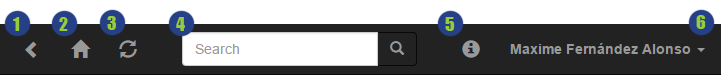
\includegraphics[scale=0.5]{Gebruikershandleiding_img/navbar.png}
\caption{De navigatiebalk die op elk scherm in de applicatie te vinden is}
\label{fig:navbar}
\end{figure}

\begin{enumerate}
\myitem De 'terug'-knop brengt u terug naar het vorige scherm.
\myitem De 'home'-knop brengt u terug naar het hoofdscherm.
\myitem De 'herlaad'-knop laadt de huidige pagina opnieuw.
\myitem De zoekfunctie is een zeer uitgebreide, gebruiksvriendelijke en interessante functie. Op het hoofdscherm filtert hij op de naam van projecten, op de project-pagina filtert hij op de naam van usecases, actoren en concepten. Voor admins (\autoref{sec:admin}) wordt er ook gefilterd op de userlist- (\autoref{fig:admin_userlist}) en teamlist-pagina (\autoref{fig:admin_teamlist}) op respectievelijk teamnamen en voor- en achternamen van gebruikers.
\myitem De 'manual'-knop brengt u ten allen tijde terug naar deze gebruikershandleiding.
\myitem Hier wordt de naam van de huidige gebruiker getoond, hier klikken geeft de 'logout'-knop weer.
\end{enumerate}

Administrators zullen een extra knop op hun navigatiebalk vinden, de 'Admin'-dropdown. Zie \autoref{sec:admin_main} voor meer uitleg hierover.

\subsection{Algemene knoppen}
Er zijn een aantal knoppen die op meerdere plaatsen in de applicatie in een gelijkaardige context gebruikt worden.\\
\begin{minipage}{0.32\textwidth}
\begin{figure}[H]
\centering

\includegraphics[scale=0.5]{Gebruikershandleiding_img/plus.png}
\caption{De 'plus' knop}
\label{fig:plus}
\end{figure}
\end{minipage}
\begin{minipage}{0.35\textwidth}
\begin{figure}[H]
\centering

\includegraphics[scale=0.5]{Gebruikershandleiding_img/min.png}
\caption{De 'min' knop}
\label{fig:min}
\end{figure}
\end{minipage}
\begin{minipage}{0.32\textwidth}
\begin{figure}[H]
\centering

\includegraphics[scale=0.5]{Gebruikershandleiding_img/edit.png}
\caption{De 'Edit' knop}
\label{fig:edit}
\end{figure}
\end{minipage}\\

De 'plus'- en 'min'-knop dienen respectievelijk voor het toevoegen en verwijderen van een tekstveld (zoals bijvoorbeeld te zien is op \autoref{fig:usecase}). Algemeen dienen groene knoppen voor het toevoegen of updaten van gegevens, terwijl rode knoppen voor het verwijderen van gegevens of annuleren van acties dienen.\\
De 'Edit'-knop (\autoref{fig:edit}) vindt u overal waar u iets kan aanpassen, bij een project zal dit de naam zijn. Maar bij een usecase kan u bijvoorbeeld, indien u daarvoor bevoegd bent, de volledige usecase aanpassen.

\section{Teamlid}
\label{sec:teamlid}
Vanaf het moment dat uw account wordt toegevoegd aan een team, kan u de projecten van dit team bekijken.

\subsection{Hoofdscherm}
\label{sec:teamlid_main}
E\'enmaal ingelogd krijgt u uw hoofdscherm te zien. Hierop vindt u alle teams waartoe u behoort met de bijhorende projecten die aan deze teams zijn toegekend. %De administrator krijgt een uitgebreider hoofdscherm te zien, dit staat beschreven in \autoref{sec:admin}.

\begin{figure}[H]
\centering
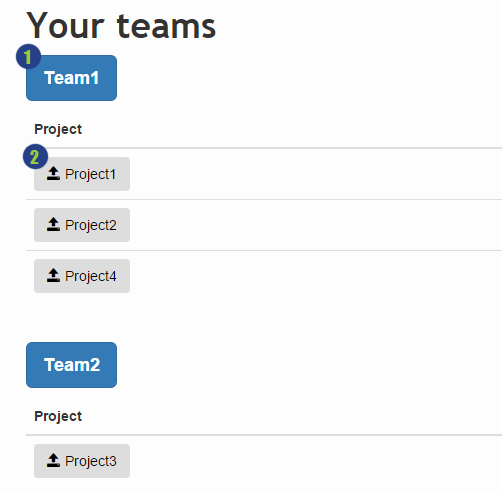
\includegraphics[scale=0.5]{Gebruikershandleiding_img/main.png}
\caption{Het hoofdscherm van een gebruiker}
\label{fig:teamlid_main}
\end{figure}

Op \autoref{fig:teamlid_main} ziet u een voorbeeld van een hoofdscherm van een gebruiker. Deze gebruiker behoort tot twee teams (Team1 en Team2), om te kijken wie er allemaal in een team zit en wat hun functies in het team zijn, klikt u op een team (bvb: \one). Ga naar \autoref{sec:teamlid_team} voor meer informatie over het teamscherm.\\
Verder zien we dat de gebruiker in een team zit met drie projecten (Team1) en een team met \'e\'en project (Team2) om zo'n projec te bekijken, kan u erop klikken (bvb \two). Ga naar \autoref{sec:teamlid_project} voor meer informatie over het projectscherm voor teamleden.

\subsection{Team}
\label{sec:teamlid_team}
Wanneer u op een team klikt, krijgt u volgend scherm te zien;

\begin{figure}[H]
\centering
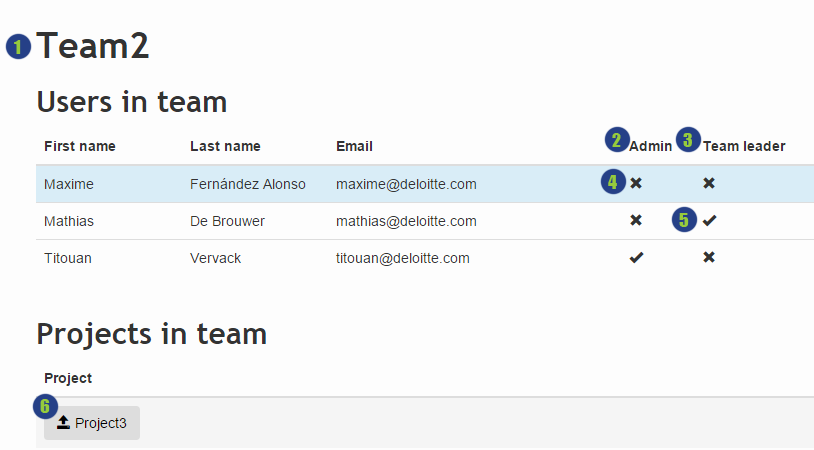
\includegraphics[scale=0.5]{Gebruikershandleiding_img/team.png}
\caption{Het teamscherm}
\label{fig:teamlid_team}
\end{figure}

Dit is het teamscherm, bovenaan staat de naam van het team (\one). Verder ziet u hier alle teamleden met hun bijhorende functies (administrator \two\ en/of teamleider \three). Deze zijn aangeduid met een kruisje of een vinkje (respectievelijk \four\ en \five).\\
Onder alle teamleden, vindt u ook alle projecten die tot dit team behoren. Ook hier kan u op een project klikken (\six) om naar de desbetreffende projectpagina te navigeren (zie \autoref{sec:teamlid_project}).


\subsection{Project}
\label{sec:teamlid_project}
\begin{figure}[H]
\centering
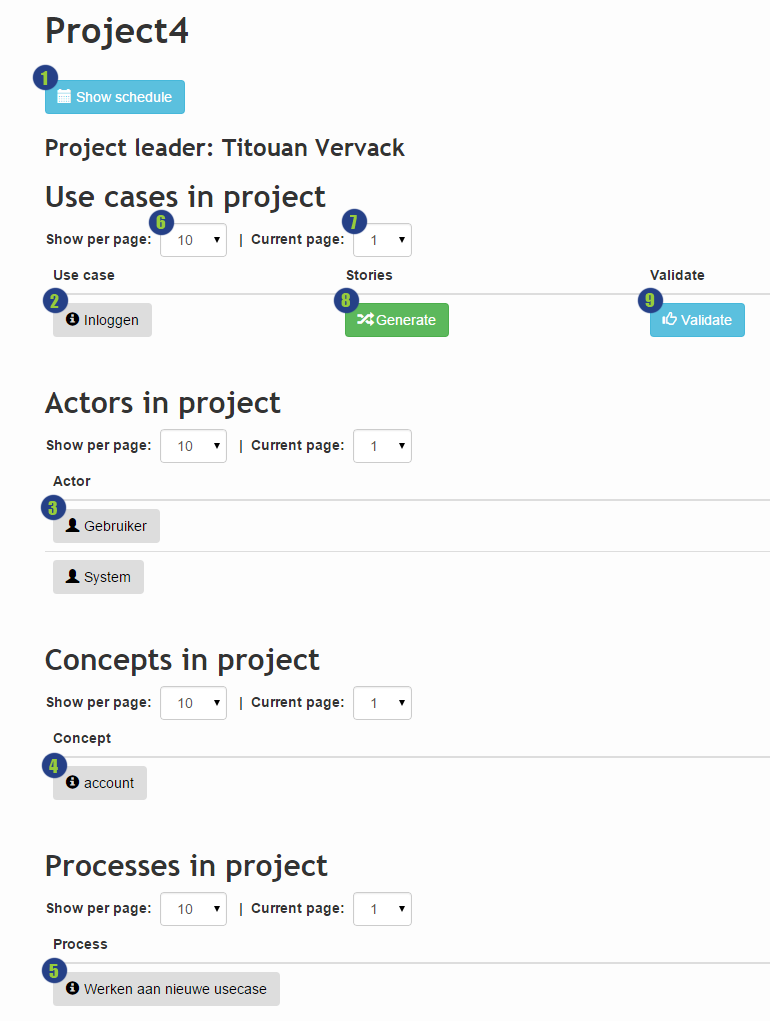
\includegraphics[scale=0.5]{Gebruikershandleiding_img/project.png}
\caption{Het project-scherm}
\label{fig:teamlid_project}
\end{figure}

Hier kan u alle usecases (\two), actoren (\three), concepten (\four) en processen (\five) van uw team bekijken. U kan deze enkel lezen, projectanalysten en -leiders kunnen deze ook aanmaken en aanpassen, zie \autoref{sec:projectlid_project} voor meer hierover. Bovenaan kan u, indien de projectleider deze heeft aangemaakt, de planning omtrent de usecases van dit project bekijken (\one\ $\rightarrow$ \autoref{fig:show_schedule}).\\
Indien er te veel entiteiten (usecases, actoren of concepten) worden weergegeven, kan u ervoor kiezen minder entiteiten per pagina te tonen. Door op \six\ te drukken kan u kiezen tussen 5, 10, 20 of alle entiteiten op \'e\'en pagina. Op 'current page' (\seven) kan u de pagina kiezen die u wenst te bekijken.\\
Het bekijken van entiteiten gebeurd door erop te klikken, u krijgt dan een overzicht van deze entiteit, zoals afgebeeld op \autoref{fig:overview_usecase}, \ref{fig:overview_actor}, \ref{fig:overview_concept} en \ref{fig:overview_process}.
Als laatste kan u ook de story genereren van een usecase (\eight\ $\rightarrow$ \autoref{fig:story}) of nagaan of usecases correct valideren, door op de '$Validate$'-knop (\nine) te drukken. Bij het valideren van een usecase zal er een venster verschijnen dat toont of de usecase al dan niet compleet volgens de regels is opgemaakt.

\begin{figure}[H]
\centering
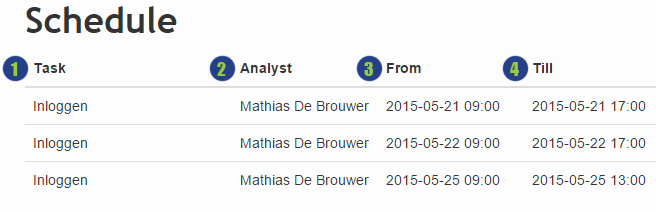
\includegraphics[scale=0.5]{Gebruikershandleiding_img/show_schedule.png}
\caption{De voorstelling van een planning}
\label{fig:show_schedule}
\end{figure}

Op \autoref{fig:show_schedule} ziet u de planning. Er wordt, in dit voorbeeld, uitsluitend aan de usecase 'Inloggen' (\one) gewerkt. Naast de naam van de usecase waaraan gewerkt moet worden, ziet u de analyst die gepland is, het werk te verrichten (\two). De laatste twee kolommen geven weer van wanneer (\three) tot wanneer (\four) er gewerkt zal moeten worden.

\begin{figure}[H]
\centering
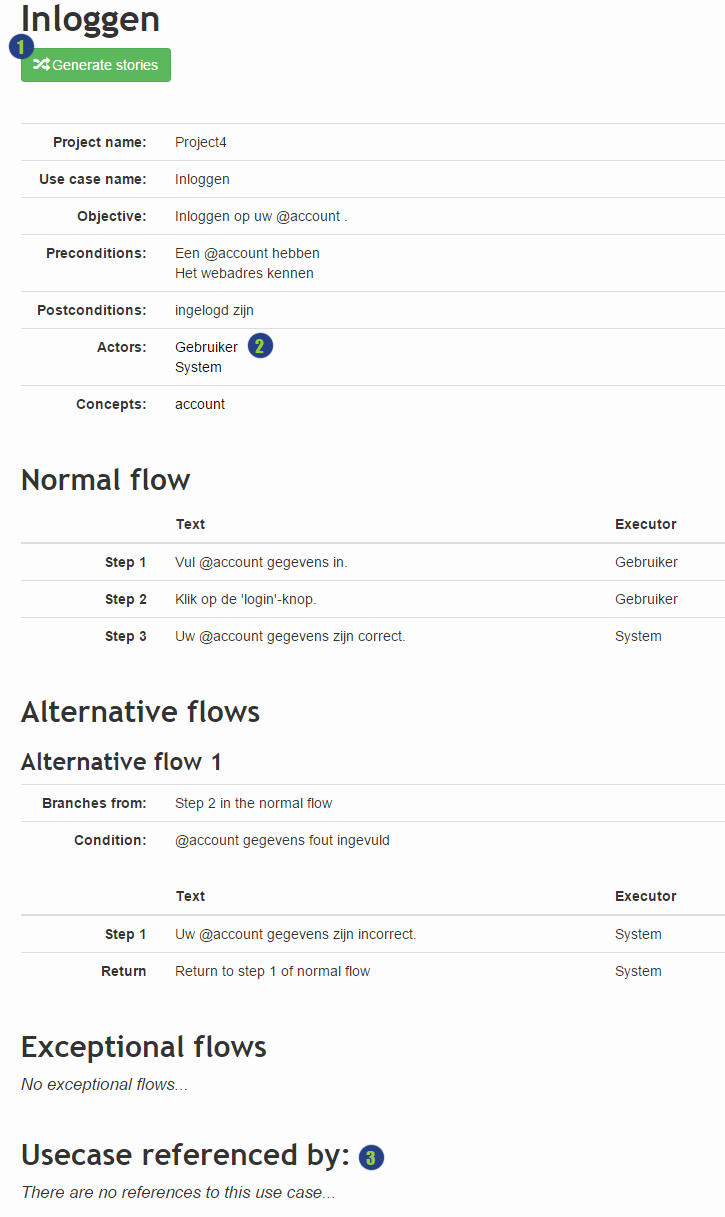
\includegraphics[scale=0.5]{Gebruikershandleiding_img/show_usecase.png}
\caption{De voorstelling van een usecase}
\label{fig:overview_usecase}
\end{figure}

Vanboven vindt u de knop '$Generate\ stories$' (\one) die de story van deze usecase genereerd. Verder ziet u hier alle condities, flows en overige informatie van de usecase, zoals deze zijn opgemaakt door een projectanalyst of -leider. Actoren en concepten die gebruikt worden in de usecase, zoals bijvoorbeeld bij \two , zijn klikbaar en zullen u naar het overzicht van de desbetreffende entiteit navigeren (zie \autoref{fig:overview_actor} en \ref{fig:overview_concept}).\\
Als laatste ziet u een overzicht van alle entiteiten waarin gerefereerd wordt naar deze usecase (\three).

\begin{figure}[H]
\centering
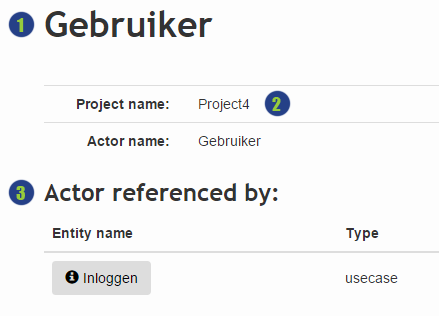
\includegraphics[scale=0.5]{Gebruikershandleiding_img/show_actor.png}
\caption{De voorstelling van een actor}
\label{fig:overview_actor}
\end{figure}

Op \autoref{fig:overview_actor} ziet u het overzicht van een actor. Dit overzicht geeft u de naam van de actor (\one) en in welk project (\two) de desbetreffende actor zich bevindt. Maar meer belangrijk ook in welke usecases, in dit project, deze actor wordt gebruikt (\three).

\begin{figure}[H]
\centering
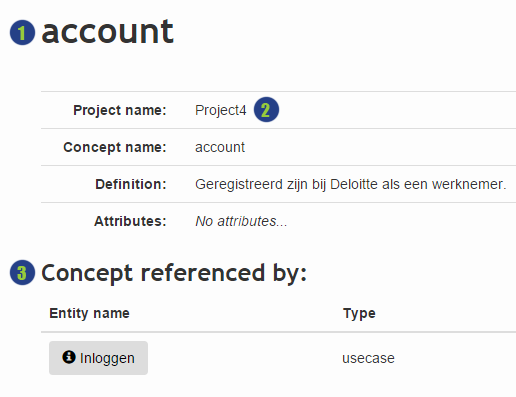
\includegraphics[scale=0.5]{Gebruikershandleiding_img/show_concept.png}
\caption{De voorstelling van een concept}
\label{fig:overview_concept}
\end{figure}

Voor concepten geldt hetzelfde als voor actoren, op \autoref{fig:overview_concept} ziet u de informatie van het concept (\one\ en \two) en in welke usecase het concept gebruikt wordt (\three).\\

\begin{figure}[H]
\centering
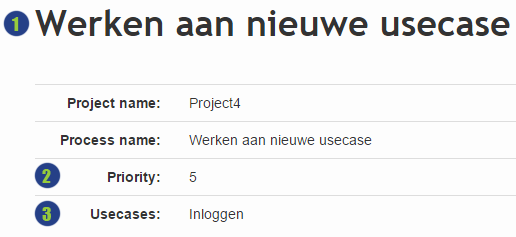
\includegraphics[scale=0.5]{Gebruikershandleiding_img/show_process.png}
\caption{De voorstelling van een proces}
\label{fig:overview_process}
\end{figure}

Het overzicht van een proces geeft onder andere de naam (\one), prioriteit (\two) en betrokken usecases (\three) weer. De prioriteit geeft weer hoe dringend dit proces is, hoe hoger de prioriteit hoe meer dringend. De betrokken usecases in een proces zijn de usecases waaraan gewerkt zal worden in dit proces.

\begin{figure}[H]
\centering
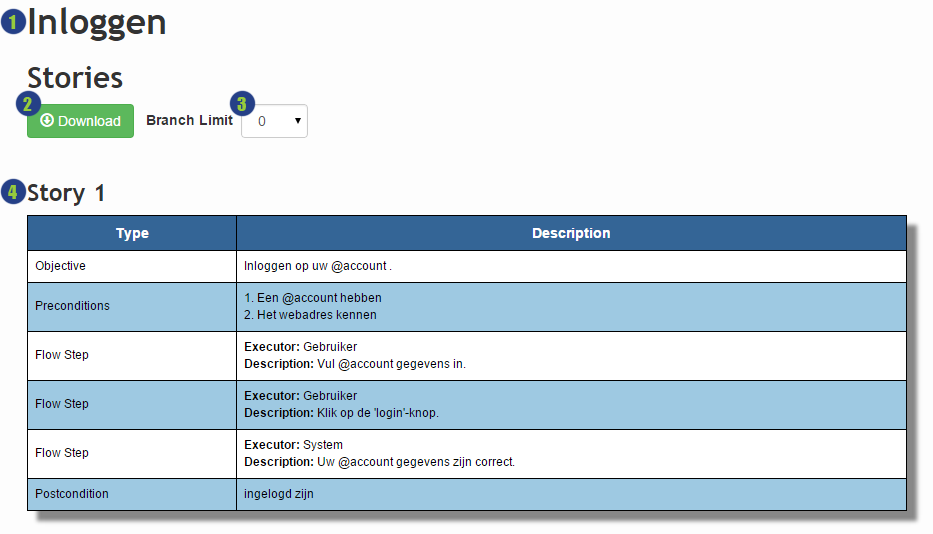
\includegraphics[scale=0.5]{Gebruikershandleiding_img/story.png}
\caption{Het 'story'-scherm}
\label{fig:story}
\end{figure}

\begin{enumerate}
\myitem De naam van de usecase waarvan u een story gegenereerd hebt.
\myitem Met \'e\'en klik op de knop download u de gegenereerde story.
\myitem De '$Branch\ Limit$' duidt op het aantal keer er naar een alternative- of exceptional-flow gegaan mag worden. Deze staat hier op nul dus wordt er niet naar de exceptional flow, zoals te zien op \autoref{fig:overview_usecase}, gegaan.
\myitem De story zelf, aangezien de '$Branch\ Limit$' op nul staat ziet u hier enkel 'Story 1', bij een hogere '$Branch\ Limit$' wordt elke mogelijke story, voor die '$Branch\ Limit$'-waarde, gegenereerd.
\end{enumerate}

\section{Projectanalyst}
\label{sec:projectlid}

Wanneer u als analyst van een project wordt aangesteld, kan u beginnen werken aan usecases, actoren, concepten en processen. Uw hoofd- en teamscherm blijven dezelfde, maar het projectscherm staat u toe aanpassingen aan te brengen.

\subsection{Hoofdscherm}
\label{sec:projectlid_main}
Het hoofdscherm van een projectanalyst is hetzelfde als die van een gewoon teamlid. Zie dus  \autoref{sec:teamlid_main} voor meer informatie.

\subsection{Team}
\label{sec:projectlid_team}
Het teamscherm van een projectanalyst is hetzelfde als die van een gewoon teamlid. Zie dus  \autoref{sec:teamlid_team} voor meer informatie.

\subsection{Project}
\label{sec:projectlid_project}
\begin{figure}[H]
\centering
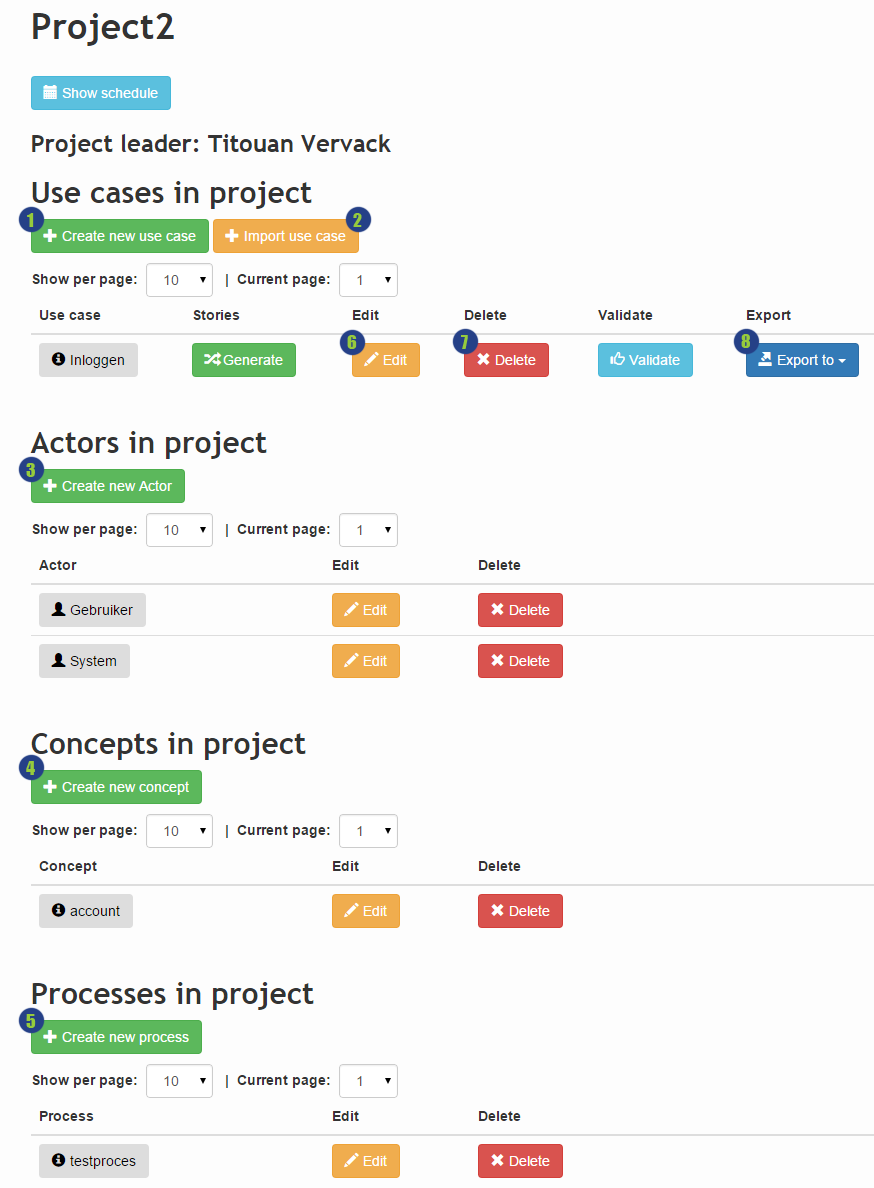
\includegraphics[scale=0.5]{Gebruikershandleiding_img/analyst_project.png}
\caption{Het project-scherm van een projectanalyst}
\label{fig:projectlid_project}
\end{figure}
U kan nieuwe usecases (\one), actoren (\three), concepten (\four) en processen (\five) aanmaken in dit project of een usecase importeren van een ander project (\two). Meer informatie hierover vindt u respectievelijk in \autoref{sec:usecase}, \ref{sec:actor}, \ref{sec:concept} en \ref{sec:process}. Op een entiteit klikken, zal u een mooi overzicht geven over de desbetreffende entiteit.\\
Een aangemaakte entiteit aanpassen kan met de 'Edit'-knop (\six) en een entiteit verwijderen kan met de 'Delete'-knop (\seven).\\
Ernaast vindt u de blauwe '$export\ to$'-knop (\eight) die u de mogelijkheid geeft om deze usecase te kopi\"eren naar een ander project waar u aan kan werken.
De overige knoppen doen hetzelfde als bij een teamlid, zoals reeds uitgelegd in \autoref{sec:teamlid_project}.

\subsubsection{Usecase}
\label{sec:usecase}
Bij het drukken op de knop 'Create new usecase' (\autoref{fig:projectlid_project}: \one) verschijnt volgend scherm (\autoref{fig:create_usecase}):

\begin{figure}[H]
\centering
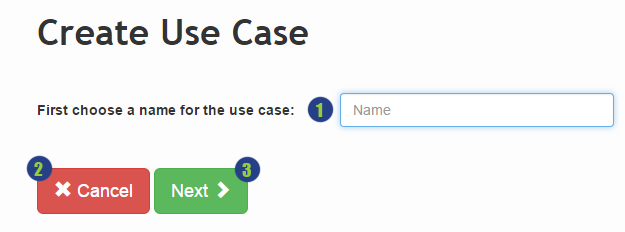
\includegraphics[scale=0.5]{Gebruikershandleiding_img/create_usecase.png}
\caption{Het tussenscherm voor het aanmaken van een usecase}
\label{fig:create_usecase}
\end{figure}

Vul bij \one\ de naam van de usecase, die u wenst aan te maken, in. Druk op 'next' (\three) om de usecase verder aan te maken. Met de 'cancel'-knop (\two) gaat alle vooruitgang in de nieuwe usecase verloren.\\

Het belangrijkste scherm van de applicatie is natuurlijk deze voor het aanmaken van de usecase.

\begin{figure}[H]
\centering
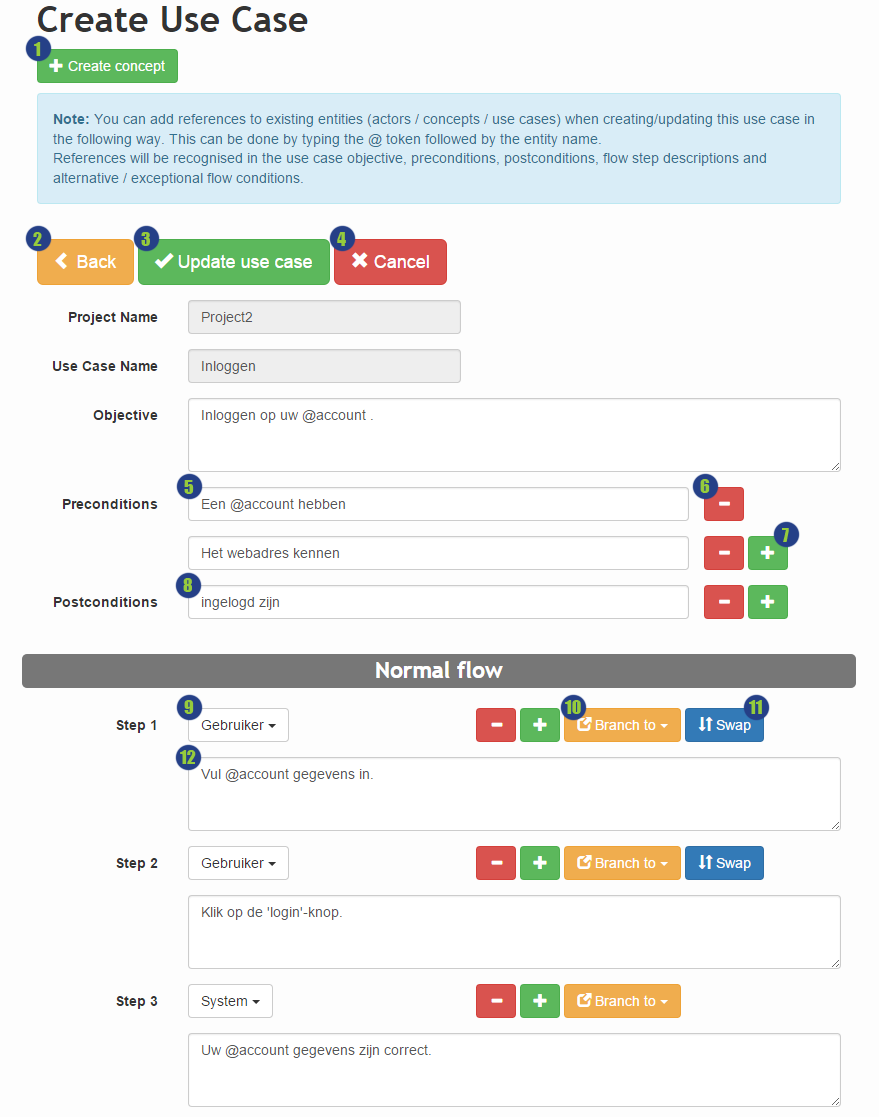
\includegraphics[scale=0.5]{Gebruikershandleiding_img/usecase.png}
\caption{Het usecase-scherm}
\label{fig:usecase}
\end{figure}

Hieronder volgt een lijst van alle opties van een usecase, zoals genummerd op \autoref{fig:usecase}.\linebreak

\begin{enumerate}
\myitem Hier kan u on-the-fly een nieuw concept aanmaken. Zie \autoref{sec:concept}.
\myitem Keer terug, zie \autoref{fig:create_usecase}.
\myitem Keer terug naar het projectscherm (\autoref{fig:projectlid_project} en verlies alle vooruitgang in deze usecase.
\myitem Het doel van deze usecase, wat moet er gebeuren?
\myitem Alle precondities van deze usecase.
\myitem De 
\includegraphics[scale=0.25]{Gebruikershandleiding_img/min.png} -knop duidt altijd op het verwijderen van een tekstveld (pre- en postcondities, normal-, alternative- en exceptional flow-stappen en meer).
\myitem De 
\includegraphics[scale=0.25]{Gebruikershandleiding_img/plus.png} -knop duidt altijd op het toevoegen van een tekstveld.
\myitem Alle postcondities van deze usecase.
\myitem Selecteer de actor van deze normal flow-stap, zie \autoref{fig:executor}.
\myitem Selecteer of deze stap al dan niet kan aftakken naar een alternative- of exceptional flow, zie \autoref{fig:branchto}.
\myitem De '$Swap$'-knop zal de positie van die stap verwisselen met de stap eronder.
\myitem De beschrijving van deze stap in de normal flow van deze usecase.
\end{enumerate}

\begin{figure}[H]
\centering
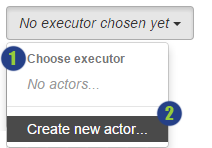
\includegraphics[scale=0.5]{Gebruikershandleiding_img/executor.png}
\caption{De 'Choose executor'-dropdown, die toelaat om actoren toe te voegen of aan te maken}
\label{fig:executor}
\end{figure}

Bij \one\ staan alle beschikbare actoren en indien u een andere actor als executor (uitvoerder)
van deze stap wil kiezen, kan u een nieuwe actor aanmaken bij puntje \two.

\begin{figure}[H]
\centering
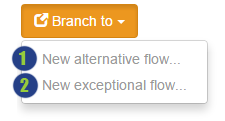
\includegraphics[scale=0.5]{Gebruikershandleiding_img/branchto.png}
\caption{De 'Branch to'-dropdown, die toelaat om alternative- en exceptional flows toe te voegen}
\label{fig:branchto}
\end{figure}

\begin{enumerate}
\myitem Deze stap kan vertakken naar een nieuwe alternative flow, zie \autoref{fig:altflow}.
\myitem Deze stap kan vertakken naar een nieuwe exceptional flow, zie hiervoor \autoref{fig:excepflow}.
\end{enumerate}

De user interface van alle flows vertoont gelijkaardigheden. Zoals de rode en groene knoppen voor het toevoegen van stappen, het kiezen van een actor en het beschrijven van de flow in de 'Description' (zie \autoref{fig:usecase}, \autoref{fig:altflow} en \autoref{fig:excepflow}).

\begin{figure}[H]
\centering
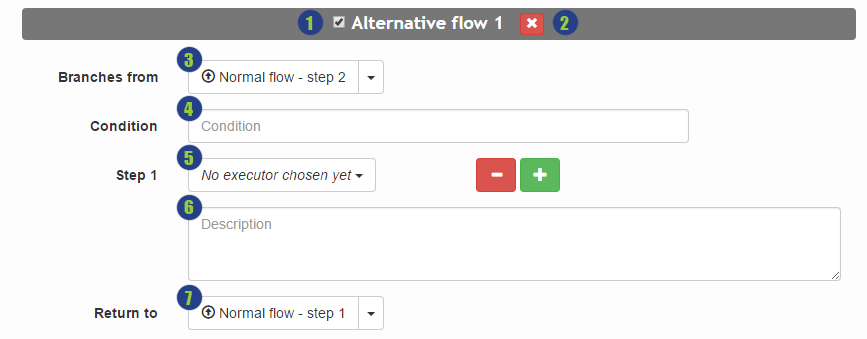
\includegraphics[scale=0.5]{Gebruikershandleiding_img/altflow.png}
\caption{Het aanmaken van een alternative flow}
\label{fig:altflow}
\end{figure}

\begin{figure}[H]
\centering
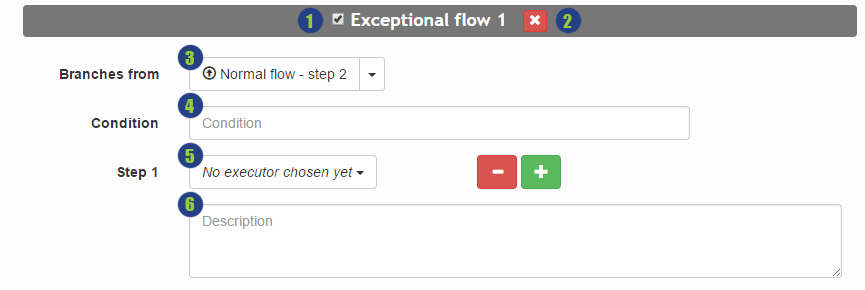
\includegraphics[scale=0.5]{Gebruikershandleiding_img/excepflow.png}
\caption{Het aanmaken van een exceptional flow}
\label{fig:excepflow}
\end{figure}

Op \autoref{fig:altflow} en \autoref{fig:excepflow} ziet u volgende puntjes:\\

\begin{enumerate}
\myitem Deze checkbox duidt aan of de flow al dan niet volledig getoond wordt.
\myitem De 
\includegraphics[scale=0.5]{Gebruikershandleiding_img/kruisje.png} -knop verwijderd deze flow.
\myitem De '$Branches\ from$'-dropdown zal automatisch wijzen naar de stap waarvan u naar deze flow bent afgetakt, maar deze kan u achteraf nog wijzigen.
\myitem De conditie waaraan moet voldaan worden vooraleer er in deze flow terecht mag gekomen worden.
\myitem Het kiezen van de actor van deze stap in de flow (zie \autoref{fig:executor}).
\myitem De beschrijving van deze stap in de flow.
\end{enumerate}

Op \autoref{fig:altflow} ziet u nog een bijkomend puntje \seven, duidend op de '$Return\ to$'-dropdown. Deze dropdown laat u toe de stap van de normal flow te kiezen waarnaar u wenst terug te keren na afloop van deze flow (zie \autoref{fig:returnto}).

\begin{figure}[H]
\centering
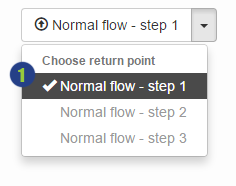
\includegraphics[scale=0.5]{Gebruikershandleiding_img/returnto.png}
\caption{De 'return to' dropdown, deze laat toe om terug te keren naar een andere stap in de usecase}
\label{fig:returnto}
\end{figure}

Op \autoref{fig:returnto} ziet u de '$Return\ to$'-dropdown box, \one\ toont hoe u een alternative flow kan laten terugkeren naar een stap in de normal flow.\\

Na het vervolledigen van uw usecase, kan u zoals een teamlid een overzicht krijgen door op de desbetreffende usecase te klikken, zie \autoref{fig:overview_usecase}. Het enige verschil is dat u bovenaan, naast de '$Generate\ stories$'-knop, een '$Edit$'- en '$Delete$'-knop zal vinden.


\subsubsection{Actor}
\label{sec:actor}
Het aanmaken van een nieuwe actor is zeer eenvoudig, u moet enkel de naam invullen. Zie \autoref{fig:actor}.\\

\begin{figure}[H]
\centering

\includegraphics[scale=0.5]{Gebruikershandleiding_img/actor.png}
\caption{Het toevoegen van een nieuwe actor}
\label{fig:actor}
\end{figure}

Ook bij een actor is het enige verschil, in vergelijking met het overzicht van een gewoon teamlid (\autoref{fig:overview_actor}), dat er een '$Edit$'- en '$Delete$'-knop bijkomen.

\subsubsection{Concept}
\label{sec:concept}
\begin{figure}[H]
\centering
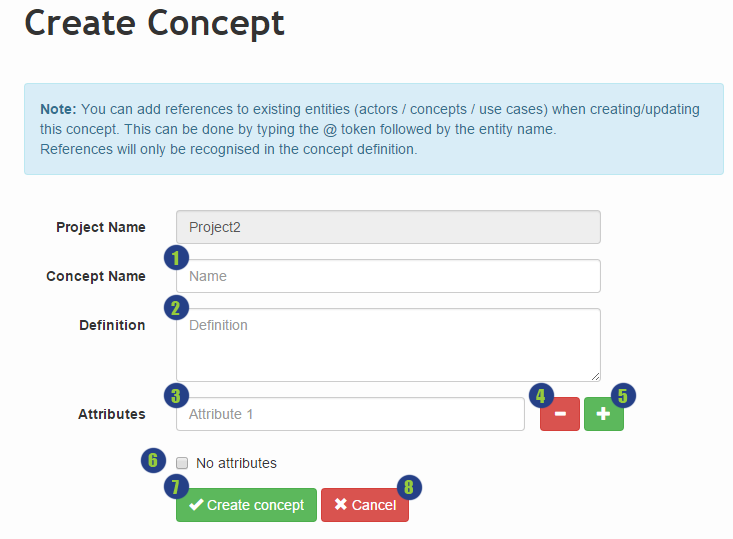
\includegraphics[scale=0.5]{Gebruikershandleiding_img/concept.png}
\caption{Het concept-scherm}
\label{fig:concept}
\end{figure}

Op \autoref{fig:concept} ziet u hoe een concept wordt aangemaakt, de figuur duidt volgende zaken aan:
\begin{enumerate}
\myitem De naam van het concept.
\myitem De definitie van dit concept, waarmee later door middel van een @-teken naar dit concept gerefereerd kan worden.
\myitem Alle attributen van dit concept.
\myitem De 
\includegraphics[scale=0.25]{Gebruikershandleiding_img/min.png} -knop dient opnieuw om een attribuut te verwijderen, dit zal echter enkel mogelijk zijn indien er meer dan \'e\'en attribuut is.
\myitem De 
\includegraphics[scale=0.25]{Gebruikershandleiding_img/plus.png} -knop dient opnieuw om een attribuut toe te voegen.
\myitem Deze checkbox duidt aan dat dit concept helemaal geen attributen heeft.
\myitem Maak dit concept aan.
\myitem Keer terug naar het projectscherm.
\end{enumerate}

En ook bij een concept krijg je een overzicht wanneer je op de naam klikt, zie \autoref{fig:overview_concept}, met twee nieuwe knoppen; een '$Edit$'- en een '$Delete$'-knop.

\subsubsection{Proces}
\label{sec:process}

\begin{figure}[H]
\centering
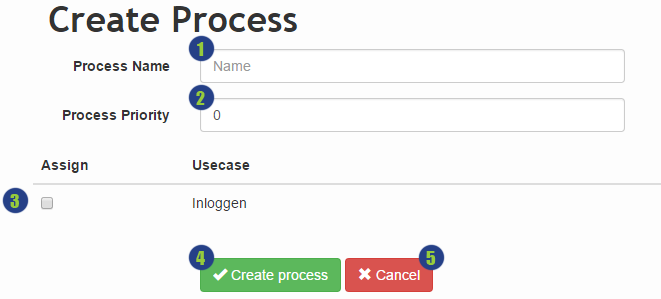
\includegraphics[scale=0.5]{Gebruikershandleiding_img/process.png}
\caption{Het proces-scherm}
\label{fig:process}
\end{figure}

\hyperref[fig:process]{Figuur \ref{fig:process}} duidt volgende zaken aan:
\begin{enumerate}
\myitem De naam van het proces dat u wenst aan te maken.
\myitem De prioriteit van dit proces, hoe hoger, hoe sneller dit proces afgewerkt moet worden.
\myitem Hier ziet u alle bestaande usecases in dit project en kan u ze toevogen aan dit proces.
\myitem Maak dit proces aan.
\myitem Keer terug naar het projectscherm.
\end{enumerate}

Klikken op het aangemaakte proces op het projectscherm, geeft u opnieuw een overzicht (zie \autoref{fig:overview_process}), maar met een '$Edit$'- en een '$Delete$'-knop.

\section{Teamleider}
\label{sec:teamleider}
Bij het aanmaken van een team door een administrator, wordt een teamleider aangesteld. Een teamleider kan vervolgens gebruikers toevoegen aan zijn team. Teamleden kunnen dan de inhoud van alle usecases, actoren en concepten van de projecten van dit team bekijken.

\subsection{Hoofdscherm}
\label{sec:teamleider_main}
Het hoofdscherm van een teamleider is hetzelfde als die van een gewoon teamlid. Zie dus \autoref{sec:teamlid_main} voor meer informatie.

\subsection{Team}
\label{sec:teamleider_team}

Het bekijken van een team biedt, in vergelijking met een teamlid, een hoop extra opties. Op \autoref{fig:teamleider_team} ziet u hoe de naam van een team aangepast kan worden (\one), gebruikers aan een team kunnen toegevoegd worden (\three) en van een team kunnen verwijderd worden (\four).\\
U kan ook zelf een andere teamleider aanstellen (\two). U kan nog altijd, zoals een gewoon teamlid, alle teamleden en hun status bekijken.

\begin{figure}[H]
\centering
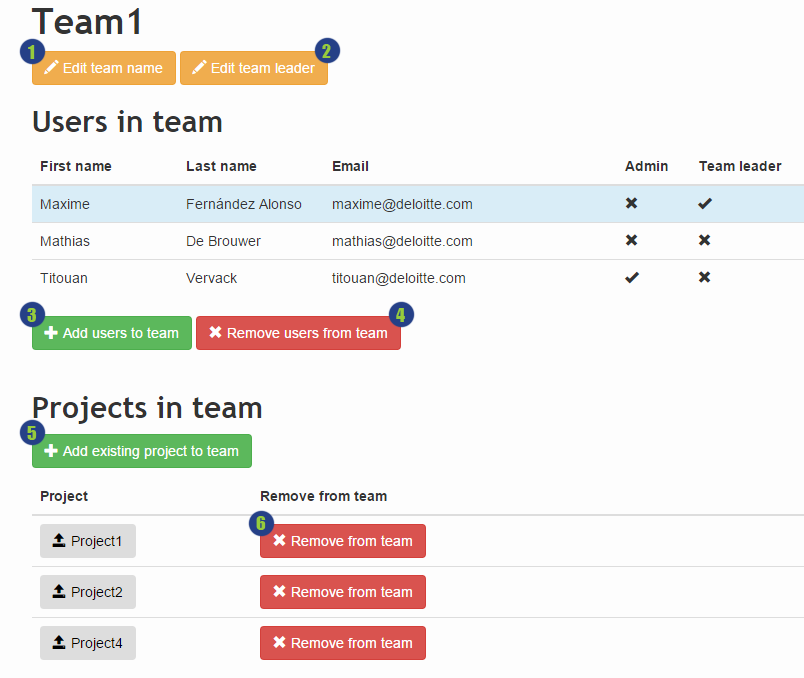
\includegraphics[scale=0.5]{Gebruikershandleiding_img/team_teamleader.png}
\caption{De voorstelling van een team, met alle opties van een teamleider}
\label{fig:teamleider_team}
\end{figure}

Indien er projecten zijn die hun maximum aantal teams nog niet bereikt hebben, kan u een bestaand project toevoegen aan uw team (\five). Ook kan u projecten van uw team bekijken en verwijderen (\six). Het project wordt in dit geval niet volledig verwijderd, het behoort dan gewoon niet meer tot het team.

\subsection{Project}
\label{sec:teamleider_project}
Het projectscherm van een teamleider is hetzelfde als die van een gewoon teamlid. Zie dus  \autoref{sec:teamlid_project} voor meer informatie.

\section{Projectleider}
\label{sec:projectleider}
Bij het aanmaken van een project door een administrator, wordt een projectleider aangesteld. Een projectleider kan vervolgens teamleden toevoegen aan het project, zodat ze zelf usecases, actoren en concepten kunnen aanmaken en aanpassen.

\subsection{Hoofdscherm}
\label{sec:projectleider_main}
Het hoofdscherm van een projectleider is hetzelfde als die van een gewoon teamlid. Zie dus \autoref{sec:teamlid_main} voor meer informatie.

\subsection{Team}
\label{sec:projectleider_team}
Het teamscherm van een projectleider is hetzelfde als die van een gewoon teamlid. Zie dus  \autoref{sec:teamlid_team} voor meer informatie.

\subsection{Project}
\label{sec:projectleider_project}
Op het projectscherm, van het project waarvan u leider bent, ziet u vier extra knoppen in vergelijking met een analyst. Deze vier knoppen (\one, \two, \three\ en \four\ op \autoref{fig:projectleider_project}) dienen respectievelijk voor het veranderen van de naam van het project, het veranderen van de projectleider, het aanpassen van de projectanalysten van dit project en het updaten van de planning van dit project.


\begin{figure}[H]
\centering
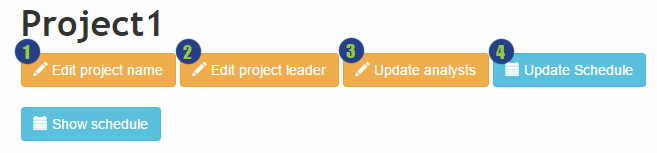
\includegraphics[scale=0.5]{Gebruikershandleiding_img/leader_project.png}
\caption{De extra opties van een projectleider op het projectscherm}
\label{fig:projectleider_project}
\end{figure}

Klikken op '$Edit\ project\ leader$' geeft u volgend scherm:
\begin{figure}[H]
\centering
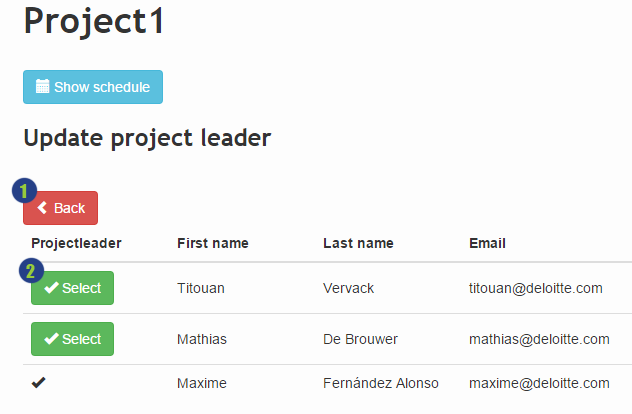
\includegraphics[scale=0.5]{Gebruikershandleiding_img/editprojectleader.png}
\caption{Wijzigen van projectleider}
\label{fig:editprojectleader}
\end{figure}
Op \autoref{fig:editprojectleader} zien we hoe u een nieuwe projectleider selecteert (\two) uit een lijst alle projectanalysten. Klik op \one\ om terug te keren naar het projectscherm.\\

Op \autoref{fig:updateanalysts} ziet u het scherm dat u krijgt indien u op '$Update\ analysts$' klikt.
\begin{figure}[H]
\centering
\includegraphics[scale=0.5]{Gebruikershandleiding_img/updateanalysts.png}
\caption{Aanstellen van projectanalysten}
\label{fig:updateanalysts}
\end{figure}
\begin{enumerate}
\myitem Deze checkbox duidt aan of een teamlid al dan niet een projectanalyst is.
\myitem Hoeveel uren zal een teamlid spenderen aan dit project?
\myitem Keer terug naar het projectscherm.
\myitem Sla uw wijzigingen op.
\end{enumerate}

Indien u de planning wenst aan te passen, klikt u op '$Update\ schedule$'. Dit doet u nadat de usecases, waaraan gewerkt moet worden, in een proces zitten.
\begin{figure}[H]
\centering
\includegraphics[scale=0.5]{Gebruikershandleiding_img/updateschedule.png}
\caption{Aanpassen van de planning van dit project}
\label{fig:updateschedule}
\end{figure}

U vult de datum in vanaf wanneer er aan het project gewerkt zal worden (\one: dd-mm-yyyy) en drukt vervolgens op '$Save$' (\two). Indien u de planning toch niet wenst aan te passen, drukt u op \three, '$Cancel$'.\\

Het aanmaken van entiteiten verloopt precies hetzelfde als bij een projectanalyst. Hiervoor verwijs ik u dus respectievelijk voor usecases, actoren, concepten en processen door naar \autoref{sec:usecase}, \ref{sec:actor}, \ref{sec:concept} en \ref{sec:process}.\\
Het overzicht van een usecase daarentegen, vertoont wel wat verschillen voor projectleiders.

\subsubsection{Usecase}
\begin{figure}[H]
\centering
\includegraphics[scale=0.5]{Gebruikershandleiding_img/leader_show_usecase.png}
\caption{De verschillende opties voor een usecase, van een projectleider}
\label{fig:leader_show_usecase}
\end{figure}

Op \autoref{fig:leader_show_usecase} zien we twee nieuwe functies die exclusief voor projectleiders en administratoren beschikbaar zijn. Hier kan u usecase-analysten aanstellen (\one) en een usecase plannen (\two).\\

Om de usecase-analysten te beheren klikt u dus op '$Update\ usecase\ analysts$', zie \autoref{fig:updateusecaseanalysts}.
\begin{figure}[H]
\centering
\includegraphics[scale=0.5]{Gebruikershandleiding_img/updateusecaseanalysts.png}
\caption{Aanstellen van usecase-analysten}
\label{fig:updateusecaseanalysts}
\end{figure}
Vink de projectanalysten aan (\one) die u wenst aan te stellen als usecase-analyst en klik vervolgens op '$Update\ changes$' (\three) om de wijzigingen door te voeren. Indien u de wijzigingen wenst te wissen, klikt u op \two.\\

Om een usecase in te plannen, klikt u op '$Schedule\ usecase$' (zie \autoref{fig:leader_show_usecase}). Vervolgens zal het volgende verschijnen;
\begin{figure}[H]
\centering
\includegraphics[scale=0.5]{Gebruikershandleiding_img/usecase_scheduling.png}
\caption{Inplannen ven een usecase}
\label{fig:usecase_scheduling}
\end{figure}
Bij \one\ vult u het aantal verwachte uren werk, en bij \two\ de prioriteit van deze usecase in. Druk vervolgens op \three\ om de usecase in te plannen of op \four\ om dit toch niet te doen.

Indien de usecase gepland is, is de '$Schedule\ usecase$'-knop verdwenen en ziet u nu het volgende;
\begin{figure}[H]
\centering
\includegraphics[scale=0.5]{Gebruikershandleiding_img/usecase_scheduled.png}
\caption{De nieuwe knoppen nadat een usecase ingepland is}
\label{fig:usecase_scheduled}
\end{figure}
\begin{enumerate}
\myitem Verwijder de planning van deze usecase.
\myitem Plan de usecase opnieuw in.
\end{enumerate}

\section{Administrator}
\label{sec:admin}
Een administrator kan enkel aangesteld worden door een andere administrator, de eerste administrator is diegene die de databank als eerste aanmaakt. Een administrator kan alles wat andere gebruikers ook kunnen. Wat enkel een administrator kan, is teams en projecten aanmaken en definitief verwijderen. Een team aanmaken gebeurd door op de 'New Team'-knop te drukken op het 'Team list'-scherm (zie \autoref{fig:admin_teamlist}: \one). Een admin kan vervolgens een project aanmaken op de team-pagina van het team die aan dat project zal werken (\autoref{fig:admin_team}: \five).

\subsection{Hoofdscherm}
\label{sec:admin_main}
Op het hoofdscherm zal een admin twee knoppen extra te zien krijgen, zoals te zien op \autoref{fig:admin_main}. Deze knoppen leiden respectievelijk naar een lijst van alle gebruikers (\one\ $\rightarrow$ \autoref{fig:admin_userlist}) en een lijst van alle teams (\two\ $\rightarrow$ \autoref{fig:admin_teamlist}).

\begin{figure}[H]
\centering
\includegraphics[scale=0.5]{Gebruikershandleiding_img/admin_main.png}
\caption{Het hoofdscherm van een administrator}
\label{fig:admin_main}
\end{figure}

Ook zal u, zoals eerder vermeld, als administrator een extra knop hebben op de navigatiebalk, de '$Admin$'-dropdown. Deze knop (\one) is een andere, snelle manier om naar de lijst van alle gebruikers (\two\ $\rightarrow$ \autoref{fig:admin_userlist}) of de lijst van alle teams (\three\ $\rightarrow$ \autoref{fig:admin_teamlist}) te navigeren.

\begin{figure}[H]
\centering
\includegraphics[scale=0.5]{Gebruikershandleiding_img/admin_navbar.png}
\caption{De navigatiebalk van een administrator}
\label{fig:admin_navbar}
\end{figure}

\begin{figure}[H]
\centering
\includegraphics[scale=0.5]{Gebruikershandleiding_img/admin_user.png}
\caption{De lijst van alle gebruikers, enkel toegankelijk door een administrator}
\label{fig:admin_userlist}
\end{figure}
Op \autoref{fig:admin_userlist} is te zien wat een admin kan doen met andere gebruikers. Zoals eerder gezegd kan een admin andere gebruikers ook administrator-rechten geven en afnemen. Dit doet hij door de checkbox (\one) al dan niet aan te vinken en nadien op '$Update\ changes$' (\four) te drukken.\\
Een gebruiker verwijderen is een onomkeerbaar proces dat u kan doen door op de rode '$remove$'-knop te drukken (\two). Met de '$Back$'-knop (\three) keert u terug naar uw hoofdscherm.


\begin{figure}[H]
\centering
\includegraphics[scale=0.5]{Gebruikershandleiding_img/admin_teamlist.png}
\caption{De lijst van alle teams, enkel toegankelijk door een administrator}
\label{fig:admin_teamlist}
\end{figure}

\hyperref[fig:admin_teamlist]{Figuur \ref{fig:admin_teamlist}} toont de lijst van alle teams.  Op dit scherm kunnen ook nieuwe teams aangemaakt worden (\one\ $\rightarrow$ \autoref{fig:create_team}). Een admin kan ook per team meer details opvragen door op een team te klikken (\two), zie \autoref{fig:admin_team} voor meer hierover.\\
Het wijzigen en verwijderen van een team gebeurt respectievelijk met de oranje '$Edit$'- (\three) en de rode '$Delete$'-knop (\four).

\begin{figure}[H]
\centering
\includegraphics[scale=0.5]{Gebruikershandleiding_img/create_team.png}
\caption{Het aanmaken van een team door op de '$New\ Team$'-knop te drukken op \autoref{fig:admin_teamlist}}
\label{fig:create_team}
\end{figure}

\subsection{Team}
\label{sec:admin_team}
Een admin kan een nieuw team aanmaken op de teamlijst-pagina, zoals te zien op \autoref{fig:admin_teamlist}.

\begin{figure}[H]
\centering
\includegraphics[scale=0.5]{Gebruikershandleiding_img/admin_team.png}
\caption{De voorstelling van een team, met alle opties van een administrator}
\label{fig:admin_team}
\end{figure}

Het bekijken van een team biedt voor een admin een hoop extra opties, in vergelijking met een gewone gebruiker. Op \autoref{fig:admin_team} ziet u hoe de naam en leider van een team aangepast kan worden (resp. \one\ en \two), gebruikers aan een team kunnen toegevoegd (\three) en van een team kunnen verwijderd worden (\four).\\
Een project toevoegen aan een team kan door een nieuw project aan te maken in dit team (\five\ $\rightarrow$ \autoref{fig:create_new_project}) of, indien het maximum aantal teams per project nog niet bereikt is, een bestaand project toe te voegen aan het team (\six\ $\rightarrow$ \autoref{fig:create_existing_project}).\\
Per project in een team heeft een administrator drie opties:
\begin{enumerate}
\myzeven Het wijzigen van de naam van het project.
\myzeven Het verwijderen van het project uit dit team.
\myzeven Het definitief verwijderen van het project.
\end{enumerate}

\begin{figure}[H]
\centering
\includegraphics[scale=0.5]{Gebruikershandleiding_img/create_new_project.png}
\caption{Toevoegen van een nieuw project aan dit team}
\label{fig:create_new_project}
\end{figure}

Op \autoref{fig:create_new_project} ziet u volgende aanwijzingen:
\begin{enumerate}
\myitem De naam van het nieuwe project.
\myitem Maak een nieuw project aan, nadat u de naam ingevuld en de projectleider geselecteerd hebt.
\myitem Annuleer het aanmaken van een nieuw project.
\myitem Selecteer een leider voor het nieuwe project, uit de lijst van alle gebruikers.
\end{enumerate}


\begin{figure}[H]
\centering
\includegraphics[scale=0.5]{Gebruikershandleiding_img/create_existing_project.png}
\caption{Toevoegen van een bestaand project aan dit team}
\label{fig:create_existing_project}
\end{figure}

Dit scherm krijgt u indien u een bestaand project wenst toe te voegen. U kiest uit de lijst van alle bestaande projecten die nog niet tot het maximum aantal teams behoren (\three). Daarna bevestigt u uw keuze door op '$Add\ selection$' te klikken (\two) of u annuleert uw keuze door op \one\ te klikken.

\subsection{Project}
\label{sec:admin_project}
Een admin kan een project aanmaken op een team-pagina (zie \autoref{fig:admin_team}).

Het projectscherm van een administrator is hetzelfde als die van een projectleider. Zie dus  \autoref{sec:projectleider_project} voor meer informatie.

\end{document}
